\section{Design}
As earlier stated the design of this solution was given thought as it had to be extensible and adaptive to changes in requirements. This section describes the process of obtaining such design and the outcome of the reflections.

\subsection{Design considerations}
An effort were made to design the system based on the five basic principles of object-oriented programming and design, SOLID. These principles applied to a system tend to make this maintainable and extendable.

\subsection{Implementation}

\begin{figure}
\centering
\includegraphics[width=0.7\linewidth]{"Images/Dependency tree"}
\caption{Dependency tree}
\label{fig:Dependencytree}
\end{figure}

\begin{figure}
\centering
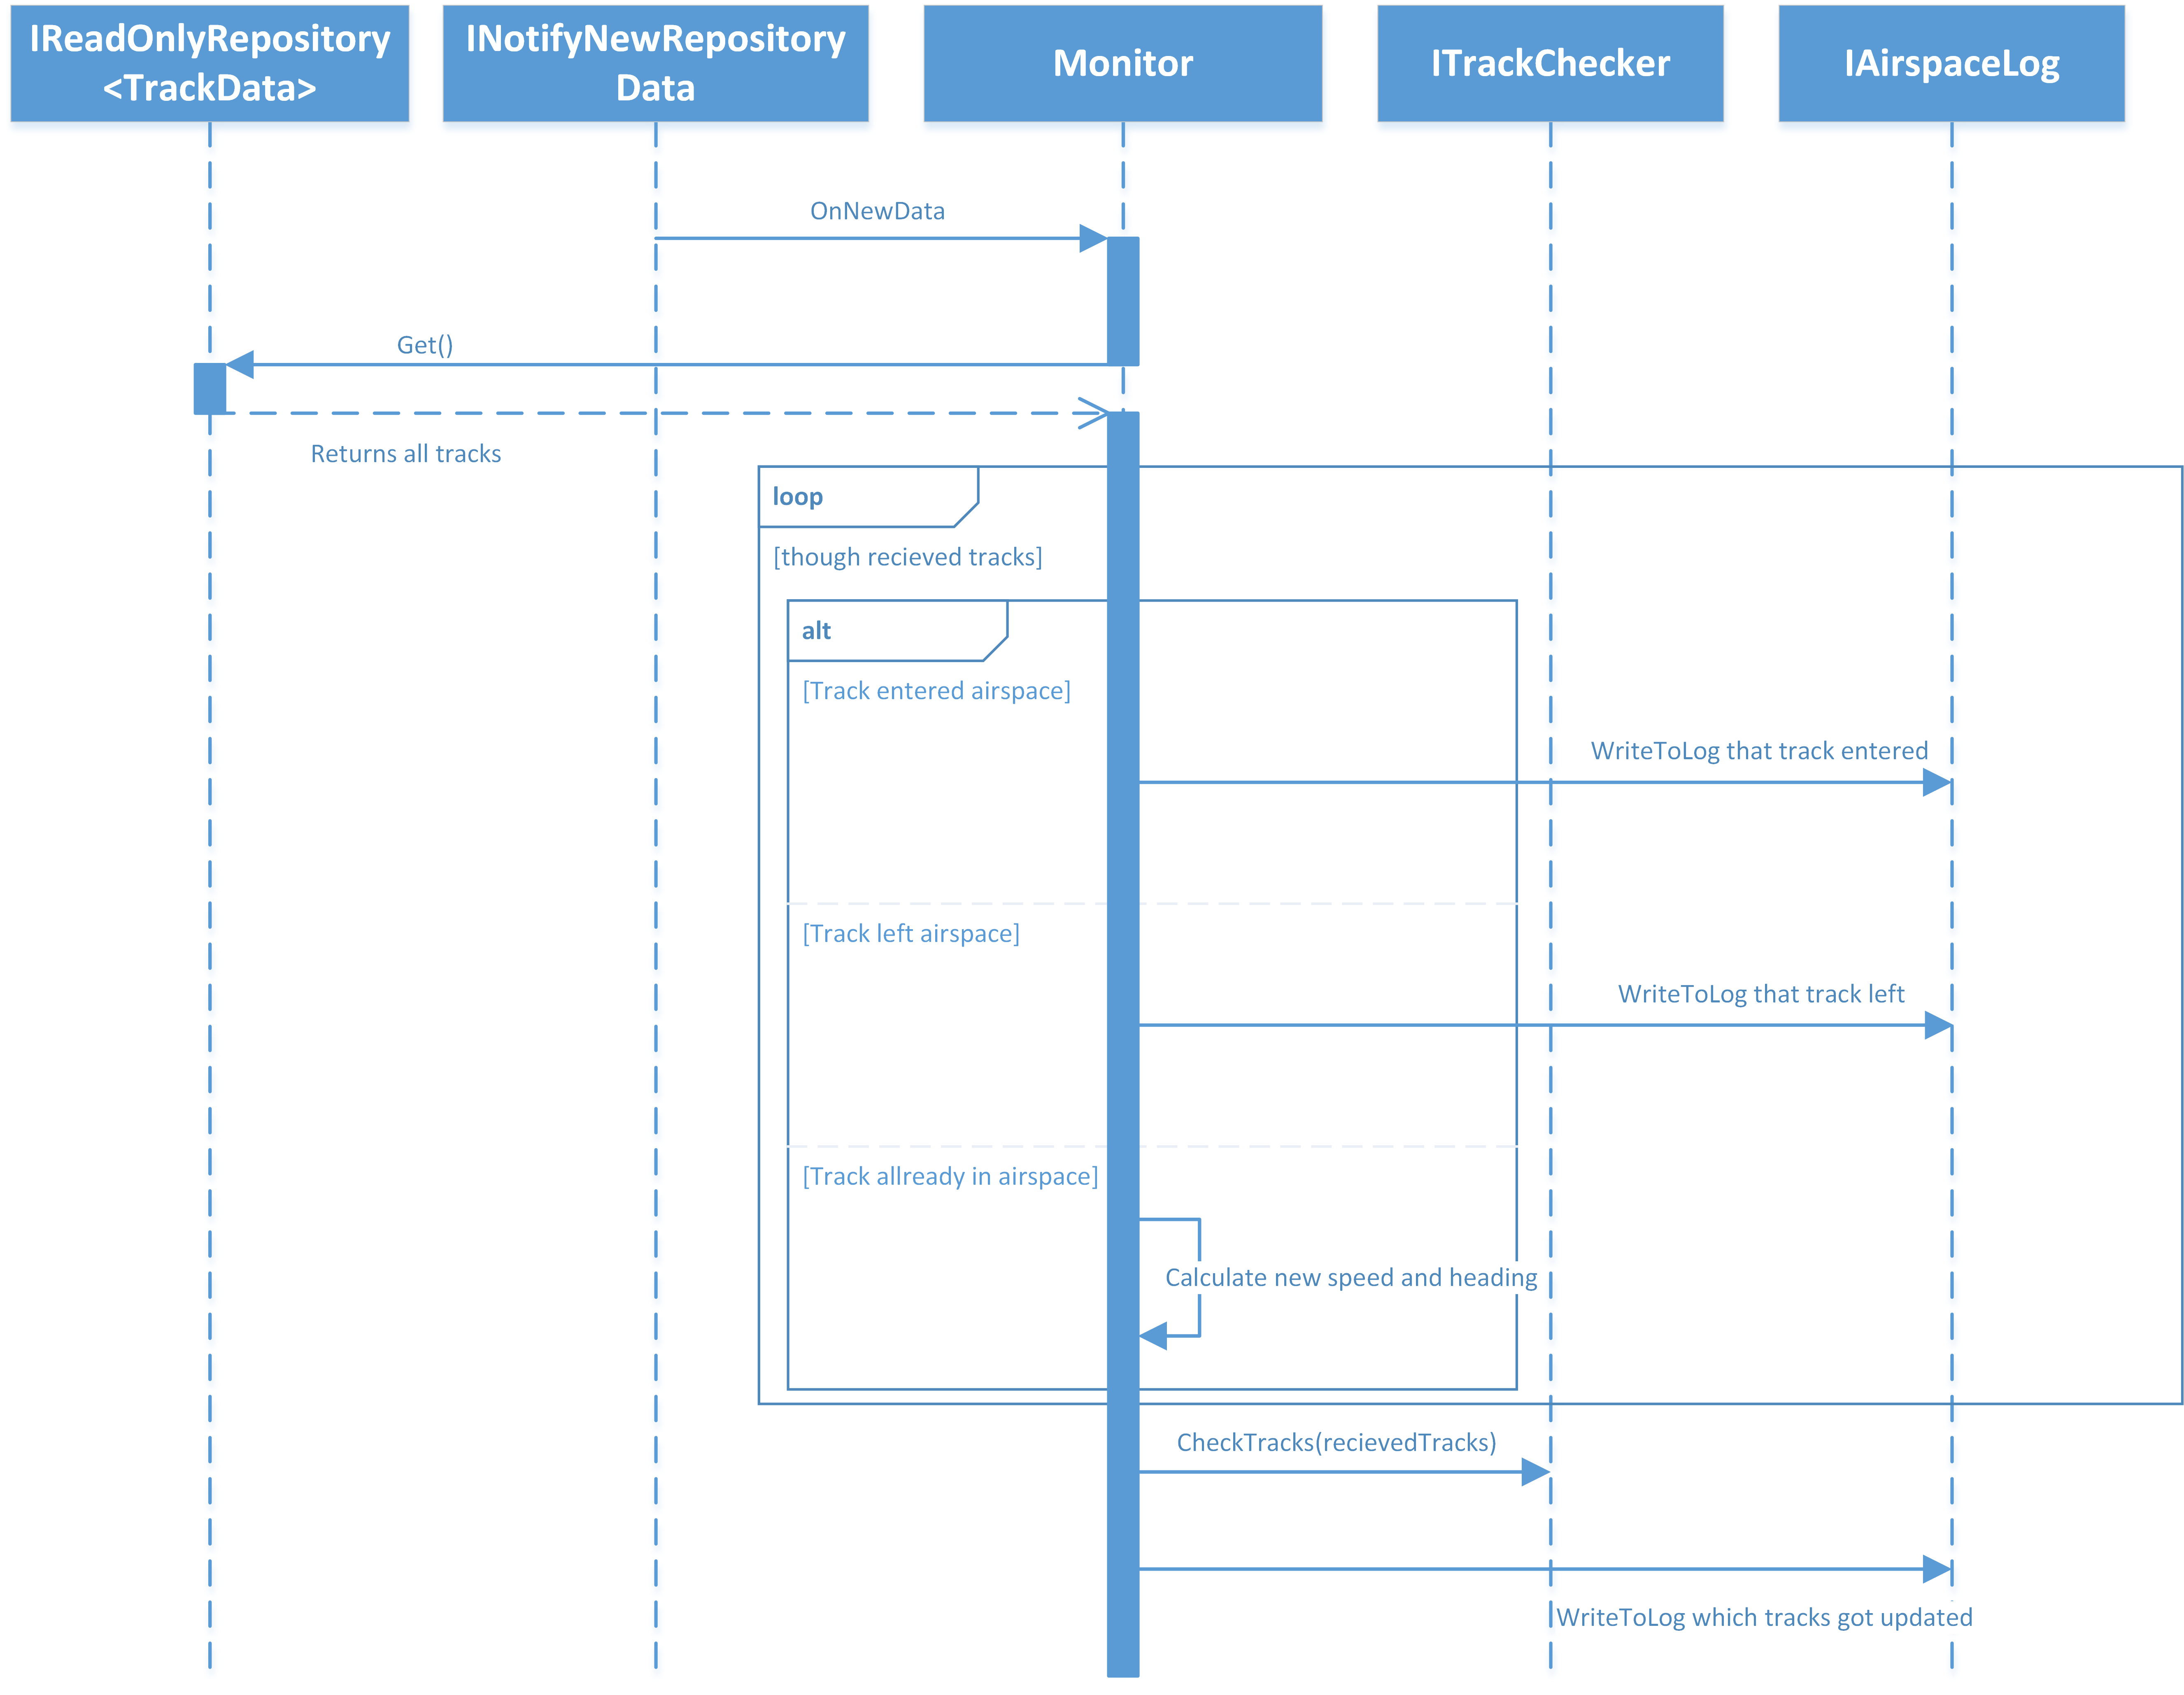
\includegraphics[width=1.0\linewidth]{Images/MonitorSeq}
\caption{Sequence diagram for monitor}
\label{fig:MonitorSeq}
\end{figure}

\begin{figure}
\centering
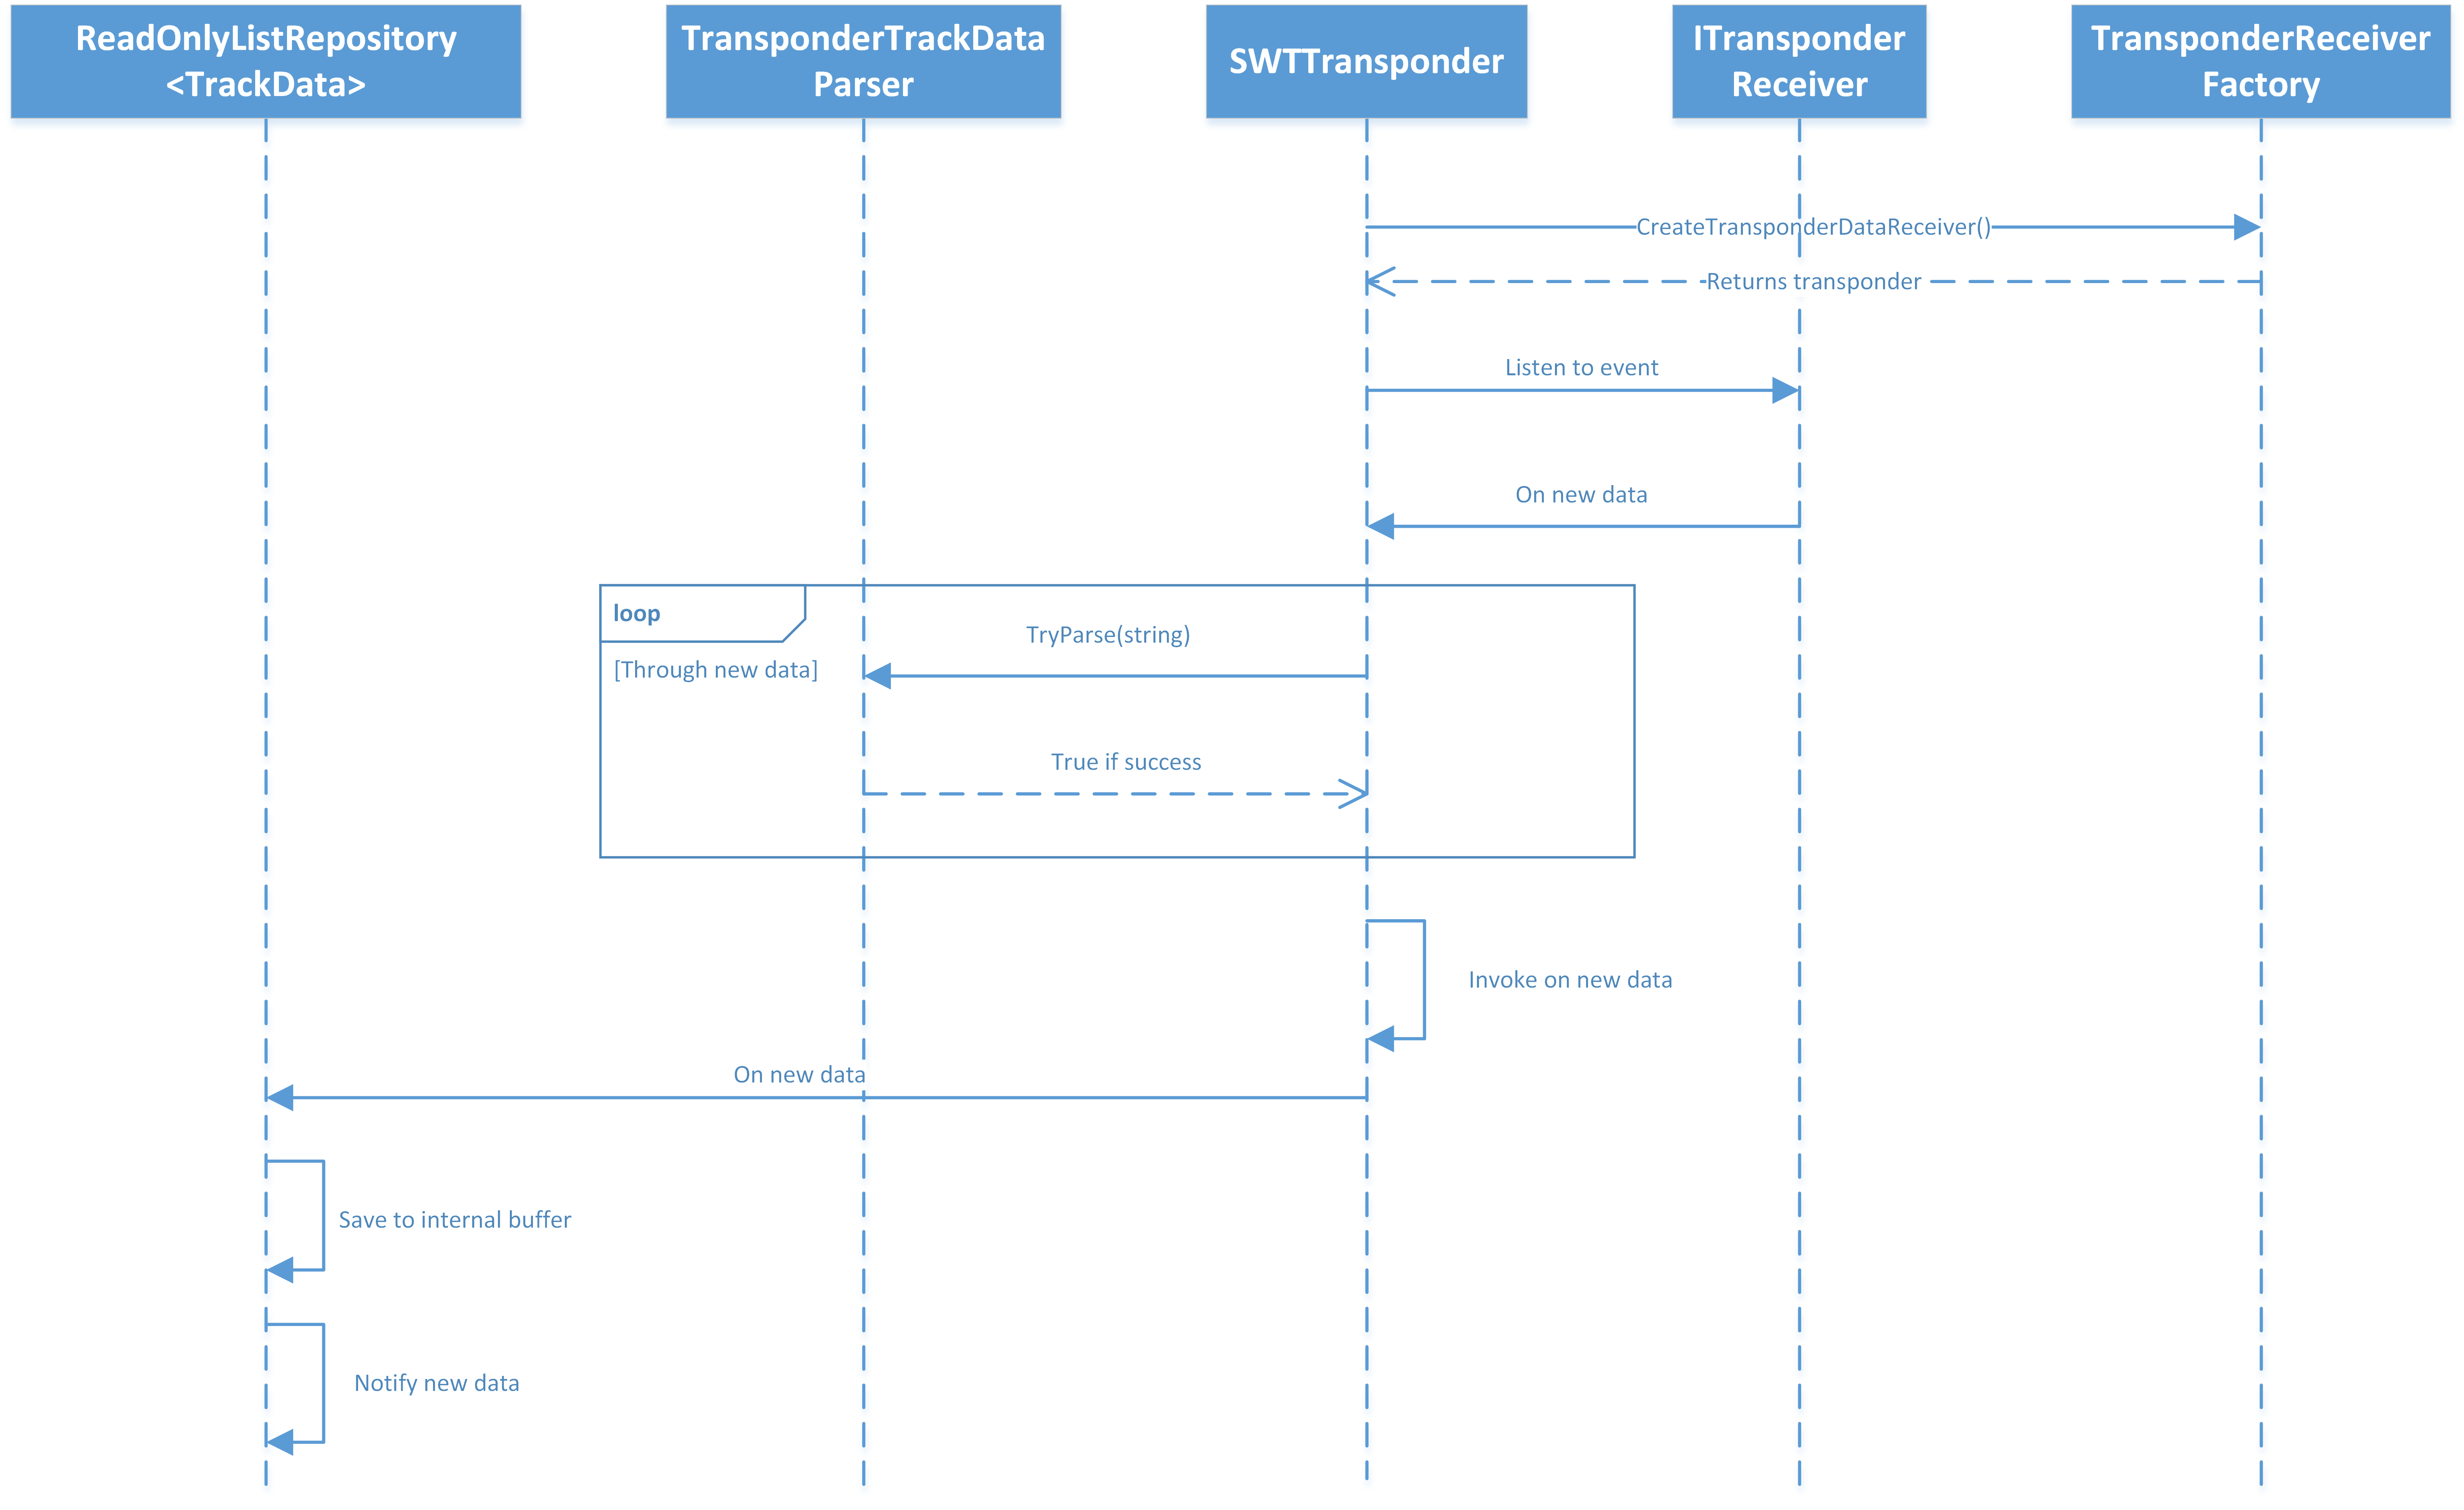
\includegraphics[width=1.0\linewidth]{Images/SWTTransponder}
\caption{Sequence diagram for SWTTransponder}
\label{fig:SWTTransponder}
\end{figure}


\clearpage
